\section{Uncertainty}
In the previous sections the algorithm results were analysed. It was assumed
that the problems were well-specified with no room for uncertainty. It was a
way to test the algorithm's behaviour and to get the idea about its
properties.

It is often impossible to specify exact values of each coefficient in the
problem. One may want to specify some of the coefficients in form of intervals
of the possible values. Then he or she is interested in robust solution taking
into account many possible scenarios of imprecision (see~[inref]). This is
possible with the DARWIN method.

Now the tests performed earlier will be extended to ``robust'' problems ---
i.e. ones with interval coefficients. Note that now it is impossible to
compare a result with the optimal solution, even assuming the supposed utility
function. However a point of reference is need in order to know what
performance can be expected from the method. The author decided to compare the
results with supposed utility function optimisation.

As a reference point for comparison result generated as follows was taken. The
whole exterior loop (see~[inref]) is left intact but in the interior loop the
goal function for evolutionary optimisation changes. Instead of optimisation
based on primary and secondary score the supposed utility function is the one
to be taken into account. This way it is possible to measure how well the DM's
preferences are inferred by the DARWIN method. And the preference gathering is
definitely most important and unique part of this method.

Like in previous sections all tests were repeated at least fifteen times and
results were averaged unless stated otherwise.

\subsection{Single run analysis}
Before evaluating performances on exemplary problems it is a good idea to
analyse single run on single problem. It can indicate interesting properties
or potential problems of the algorithm.

The problem being evaluated is a two-criteria mix problem (not that this a
problem from original DARWIN lecture given at~[ref]). Note that although the
problem has only two-criteria in its definition it has to be considered in a
space with more dimensions. This is because the supposed utility function is
defined not in the original two-criteria space (\textit{max} profit,
\textit{min} time) but rather in a quantile space (see~[inref]). The function
is defined as follows:
\begin{equation*}
\textit{max}: \hspace{0.2cm} \text{profit}^{1\%} + 3 * \text{profit}^{25\%} +
2 * \text{profit}^{50\%} - \text{time}^{1\%} - 3 * \text{time}^{25\%} - 2 *
\text{time}^{50\%}
\end{equation*}

So the space has six dimensions: $p^{1\%} \times p^{25\%} \times p^{50\%}
\times t^{1\%} \times t^{25\%} \times t^{50\%}$; $t$ is for time and $p$ for
profit.

\begin{figure}
  \centering
  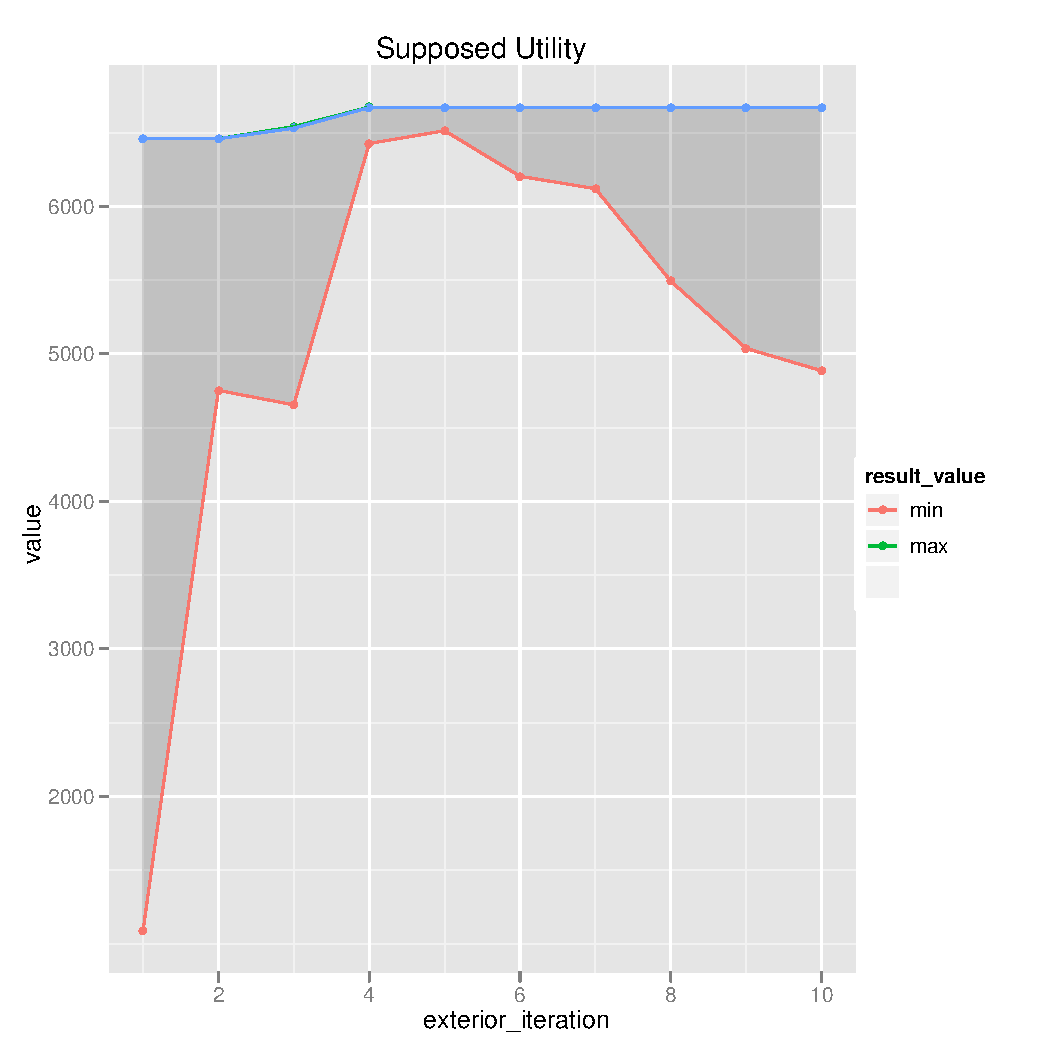
\includegraphics[width=0.8\textwidth]{exp/uncert/pres_utilouter}
  \caption{Supposed utility function in exterior loop iterations for the
    mix-problem}
  \label{pres_utilouter}
\end{figure}

Basic performance of single run is presented on
figure~\ref{pres_utilouter}. As one can see the algorithm needs only four
iteration to reach maximum value --- a point were no further improvement
occurs\footnote{This is not optimal solution to the problem. By their nature
  --- intervals and scenarios of uncertainty --- a problem from this section
  do not have a optimal value.}.

Improvements of the supposed utility function and primary score are shown on
figures~\ref{pres_utilgen_01},~\ref{pres_utilgen_03} whereas the shape of the
population on fig.~\ref{pres_utilind_01},~\ref{pres_utilind_03}. One can see
that it is easy to generate a good solution to the problem --- a solution with
the best result in given run appears in a first few generations.

Having sixth-dimensional objective space it is impossible to provide section
of this space on two-dimensional chart. However these dimensions are not
completely independent. There is a correlation between the quantiles of the
same objective. This can be observed on fig.~\ref{pres_valweight} --- showing
the movement of population during the generation on a section of objective
space or even better on fig.~\ref{pres_dm_choices} --- solutions marked by the
decision maker as ``good''.

As expected the solutions chosen by the DM are near the pareto-front. However
not all of them are part of the front. Knowing that there are four other goals
besides profit$^{50\%}$ and time$^{50\%}$ explains the phenomenon.

\begin{figure}
  \centering
  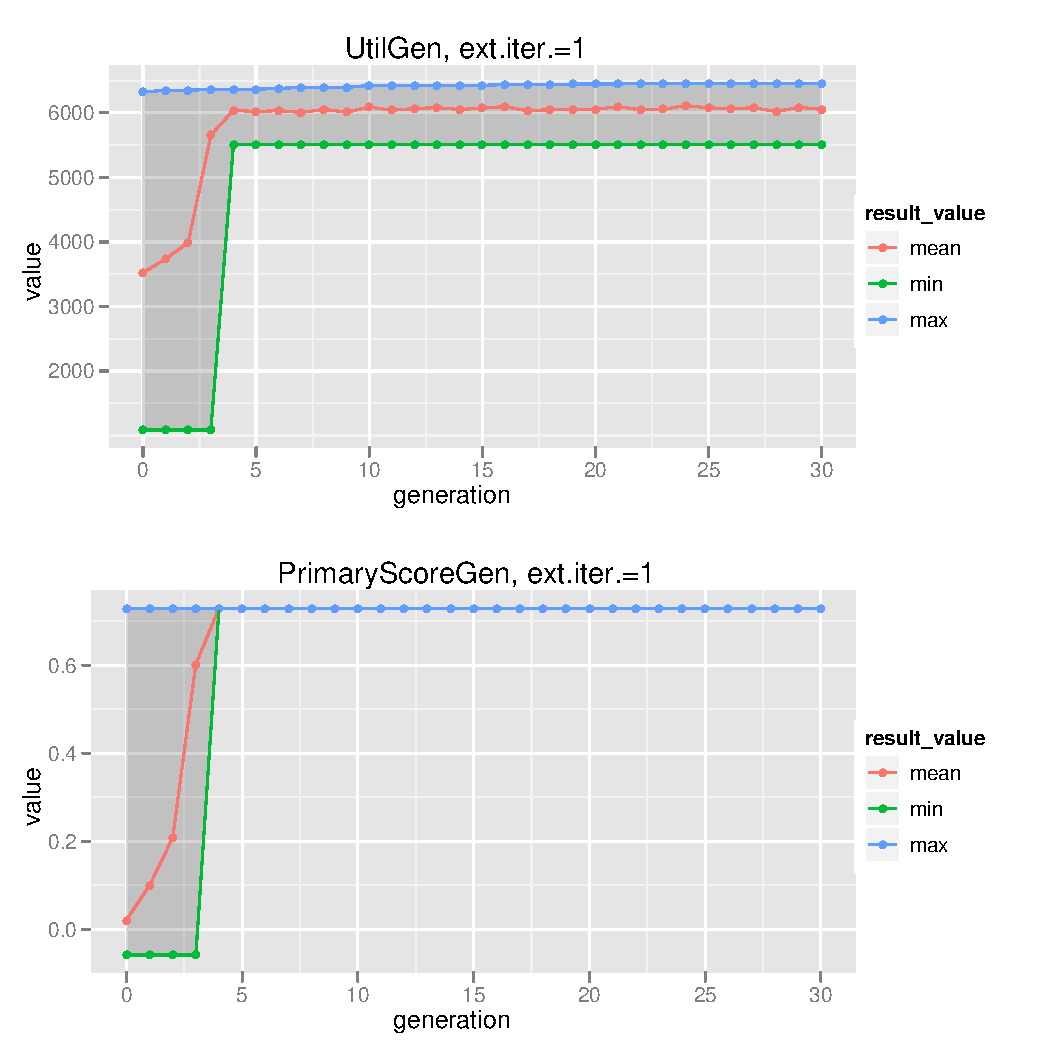
\includegraphics[width=1\textwidth]{exp/uncert/pres_utilgen_01}
  \caption{Supposed utility function and primary score improvements in an
    example run of the interior loop}
  \label{pres_utilgen_01}
\end{figure}

\begin{figure}
  \centering
  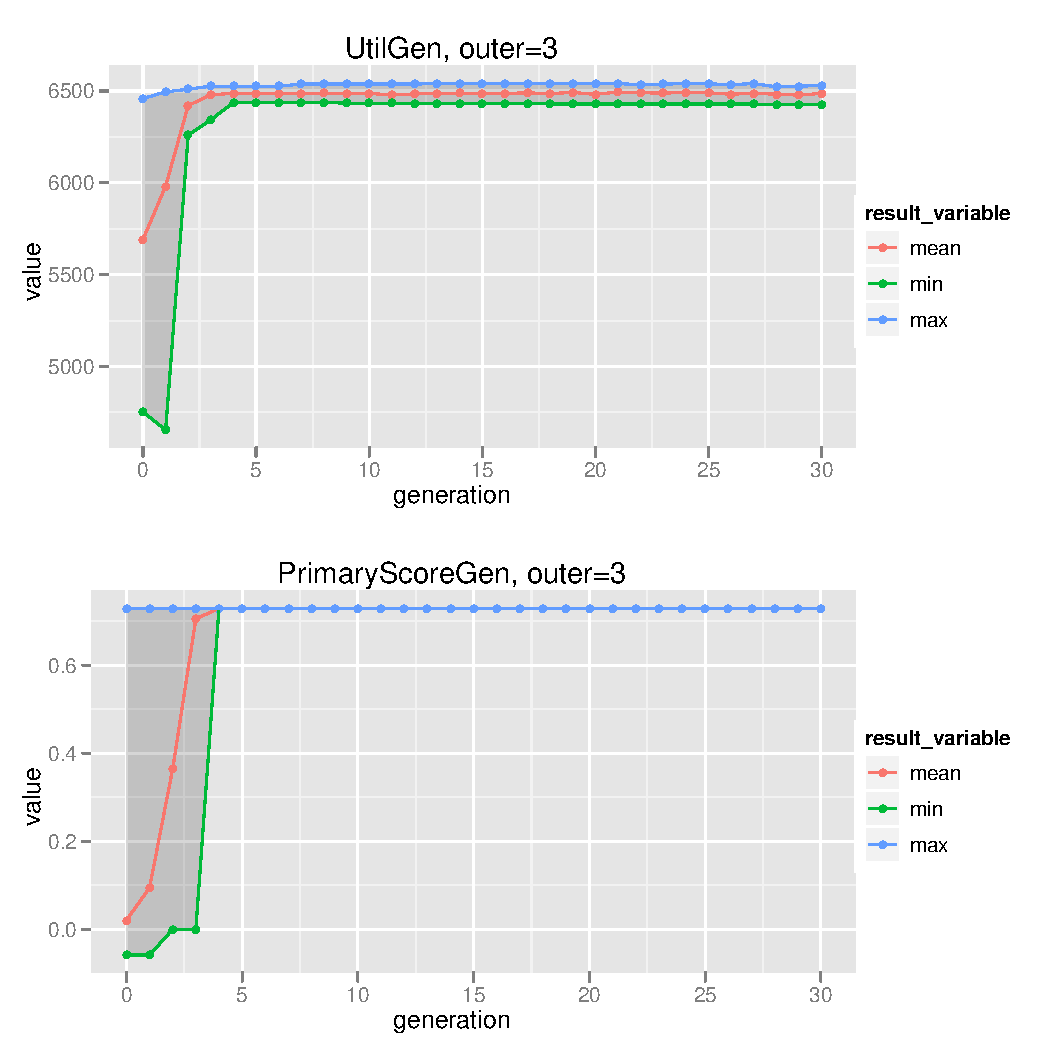
\includegraphics[width=1\textwidth]{exp/uncert/pres_utilgen_03}
  \caption{Supposed utility function and primary score improvements in an example run of the
    interior loop}
  \label{pres_utilgen_03}
\end{figure}

\begin{figure}
  \centering
  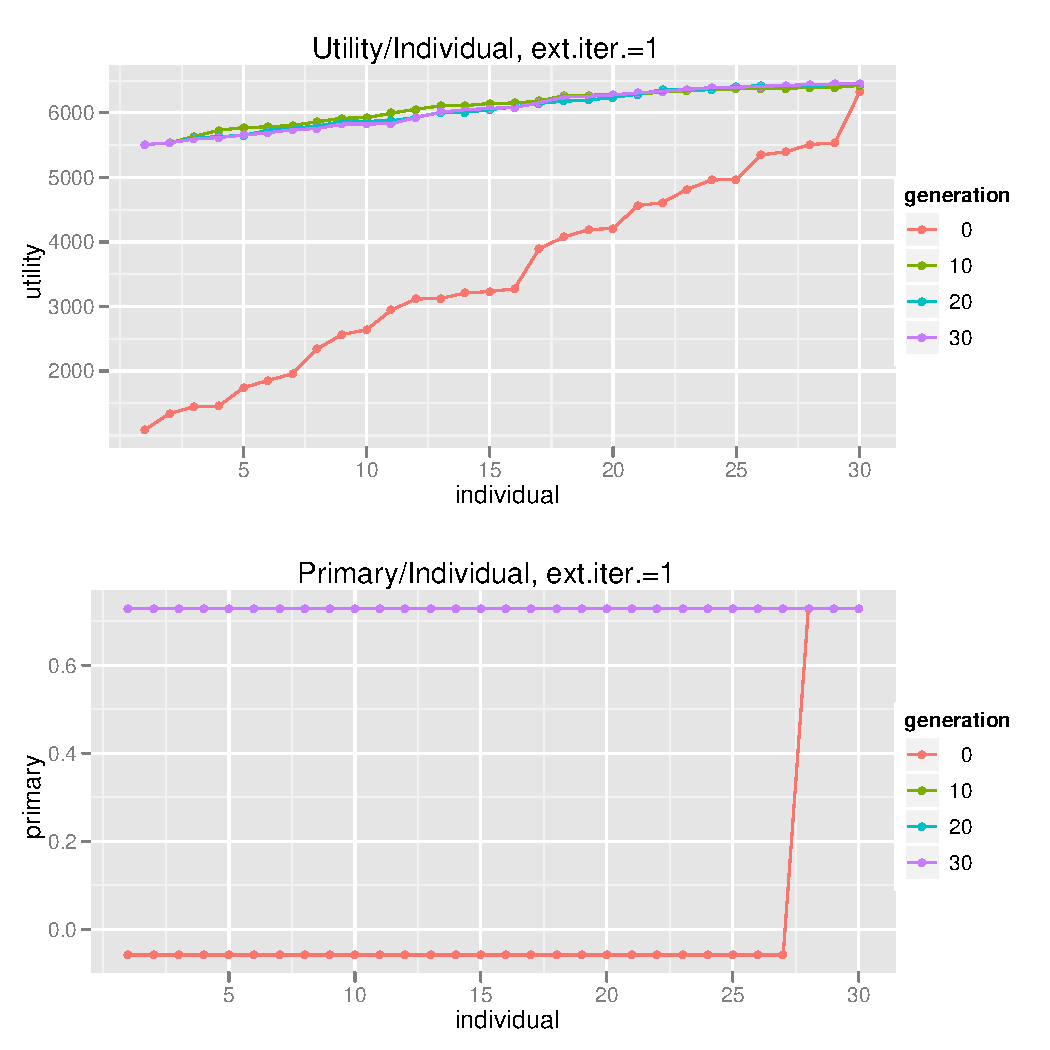
\includegraphics[width=1\textwidth]{exp/uncert/pres_utilind_01}
  \caption{Changes of the population shape in an example run of the interior
    loop}
  \label{pres_utilind_01}
\end{figure}

\begin{figure}
  \centering
  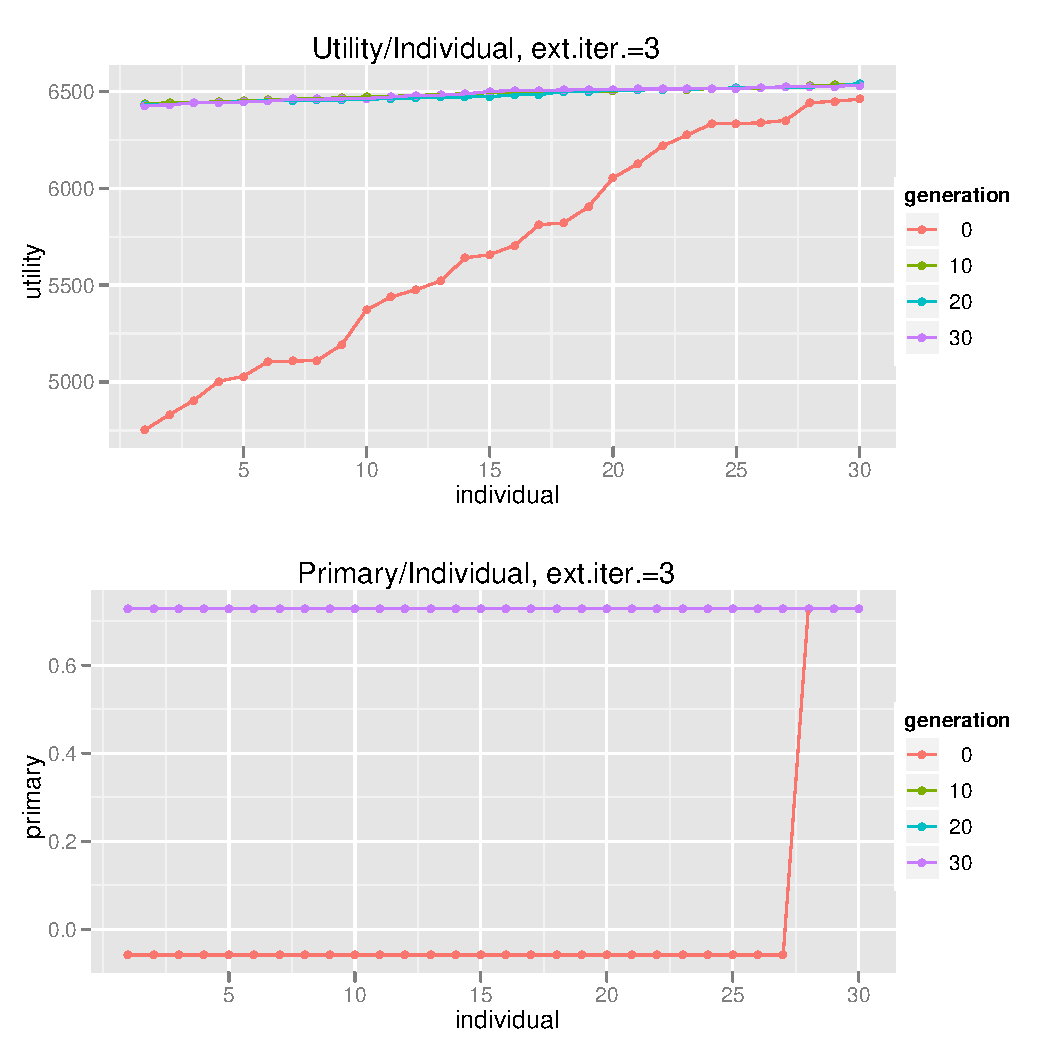
\includegraphics[width=1\textwidth]{exp/uncert/pres_utilind_03}
  \caption{Changes of the population shape in an example run of the interior
    loop}
  \label{pres_utilind_03}
\end{figure}

\begin{figure}
  \centering
  \makebox[\textwidth]{
    \subfloat{
      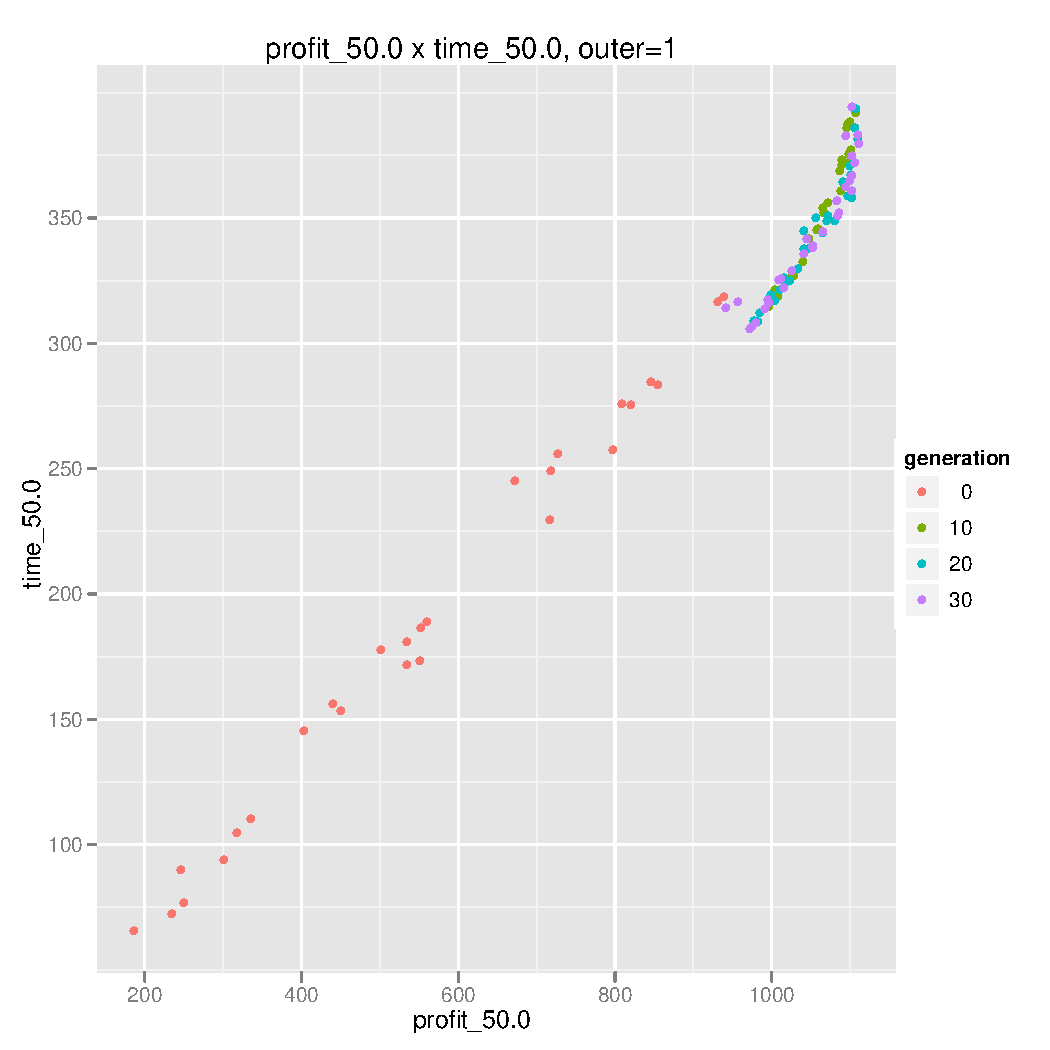
\includegraphics[scale=0.53]{exp/uncert/pres_valweight_01}
      \label{pres_valweight_01}
    }
    \subfloat{
      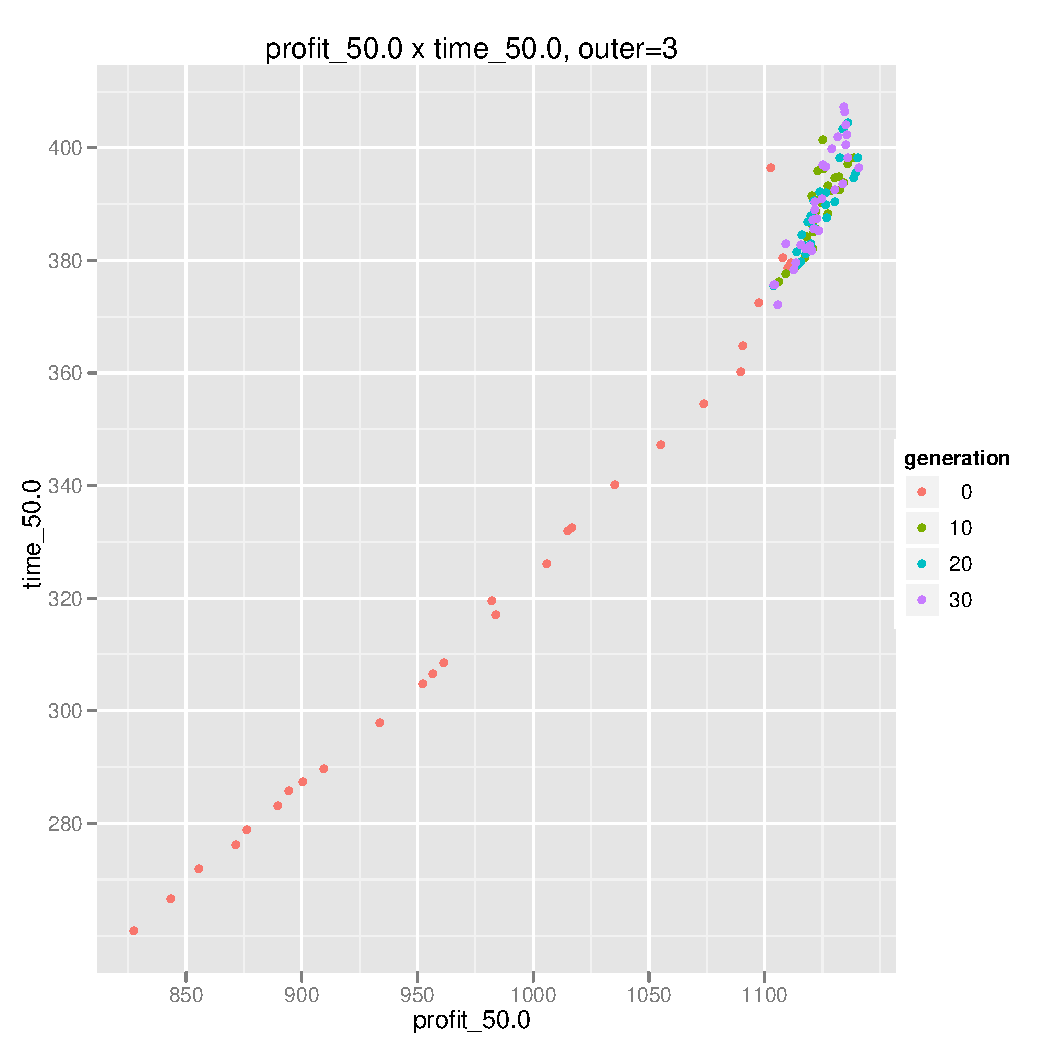
\includegraphics[scale=0.53]{exp/uncert/pres_valweight_03}
      \label{pres_valweight_03}
    }
  }
  \caption{Two-dimensional section of the objective space}
  \label{pres_valweight}
\end{figure}

\begin{figure}
  \centering
  \makebox[\textwidth]{
    \subfloat{
      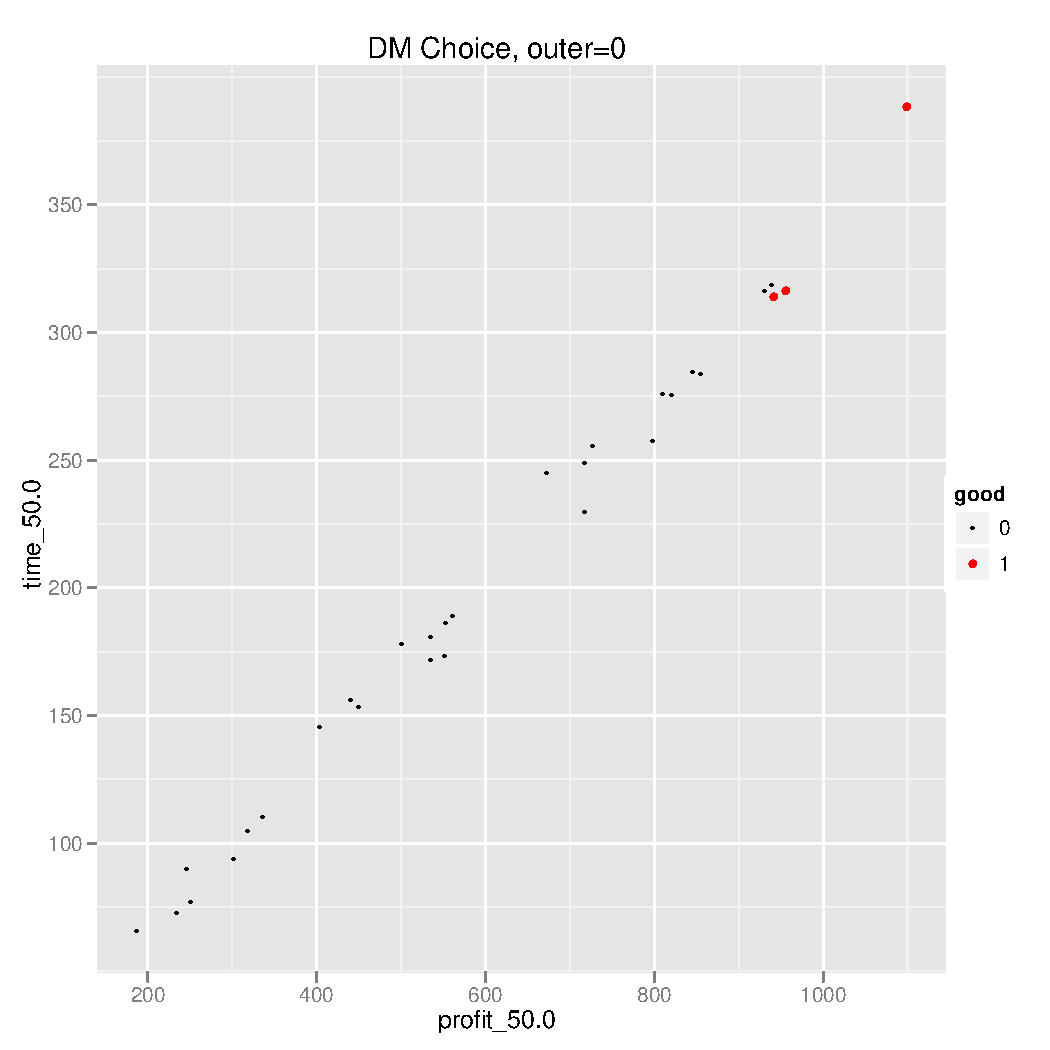
\includegraphics[scale=0.53]{exp/uncert/pres_dm_choices_01}
      \label{pres_dm_choices_01}
    }
    \subfloat{
      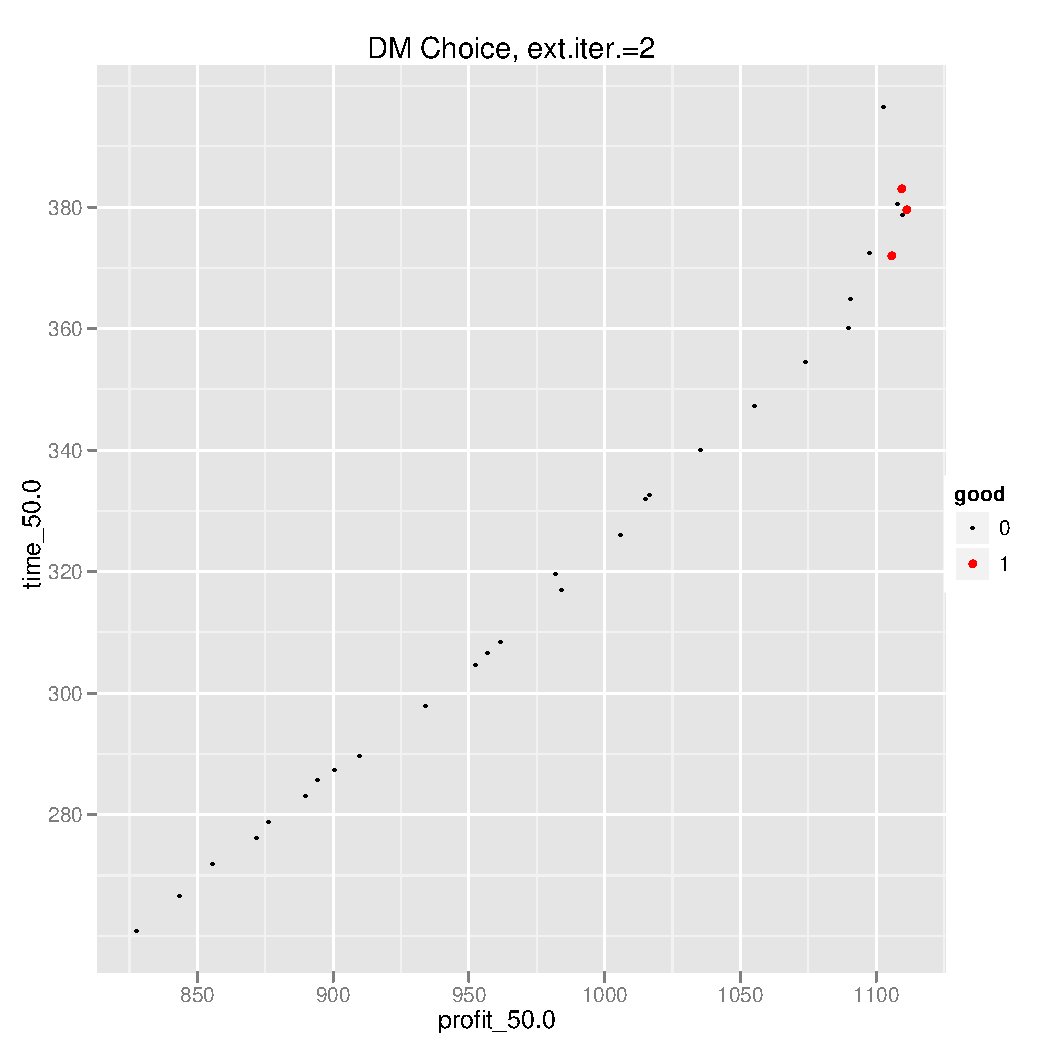
\includegraphics[scale=0.53]{exp/uncert/pres_dm_choices_03}
      \label{pres_dm_choices_03}
    }
  }
  \caption{Two-dimensional section of the objective space}
  \label{pres_dm_choices}
\end{figure}
\clearpage{}

\subsection{The performance on exemplary problems}
To see how well the DARWIN can infer the decision maker's preferences
comparison with supposed utility function is given. It section the experiments
where performed on all exemplary problems with interval coefficients --- mix
problem (also labeled as presentation problem), dtlz1 (version with four and
ten criteria) and dtlz7.

The problems were solved with default (base) values of configuration options
as well as with increased number of generation (from $30$ to $60$). Tests that
names ends with \texttt{\_rules} are using primary and secondary score; tests
with names ending with \texttt{\_supp} are using supposed utility function
value as an objective in evolutionary optimisation.

\begin{figure}
  \centering
  \makebox[\textwidth]{
    \subfloat{
      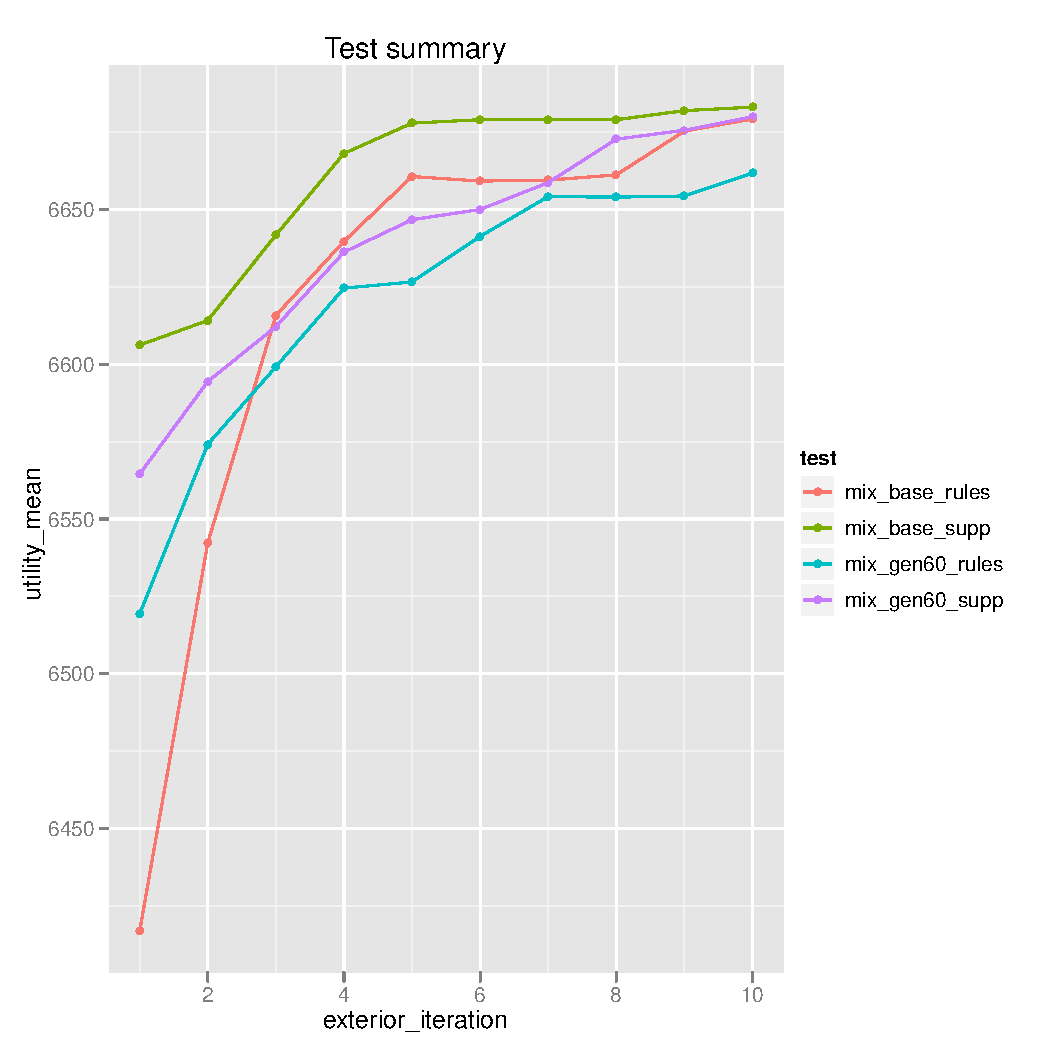
\includegraphics[scale=0.53]{exp/uncert/pres_perf1}
      \label{pres_perf1}
    }
    \subfloat{
      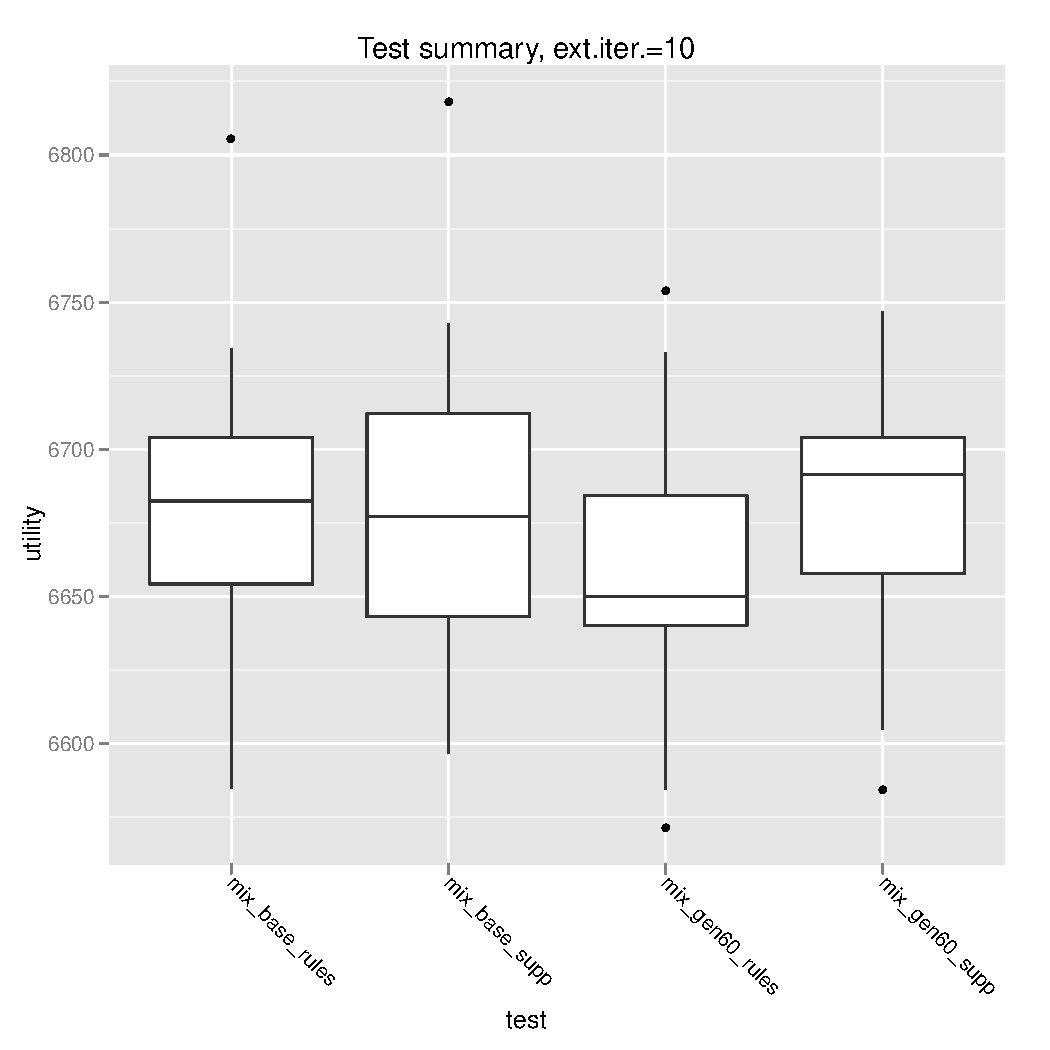
\includegraphics[scale=0.53]{exp/uncert/pres_perf1b}
      \label{pres_perf1b}
    }
  }
  \caption{Performance comparison on the mix problem}
  \label{pres_perf}
\end{figure}

\begin{figure}
  \centering
  \makebox[\textwidth]{
    \subfloat{
      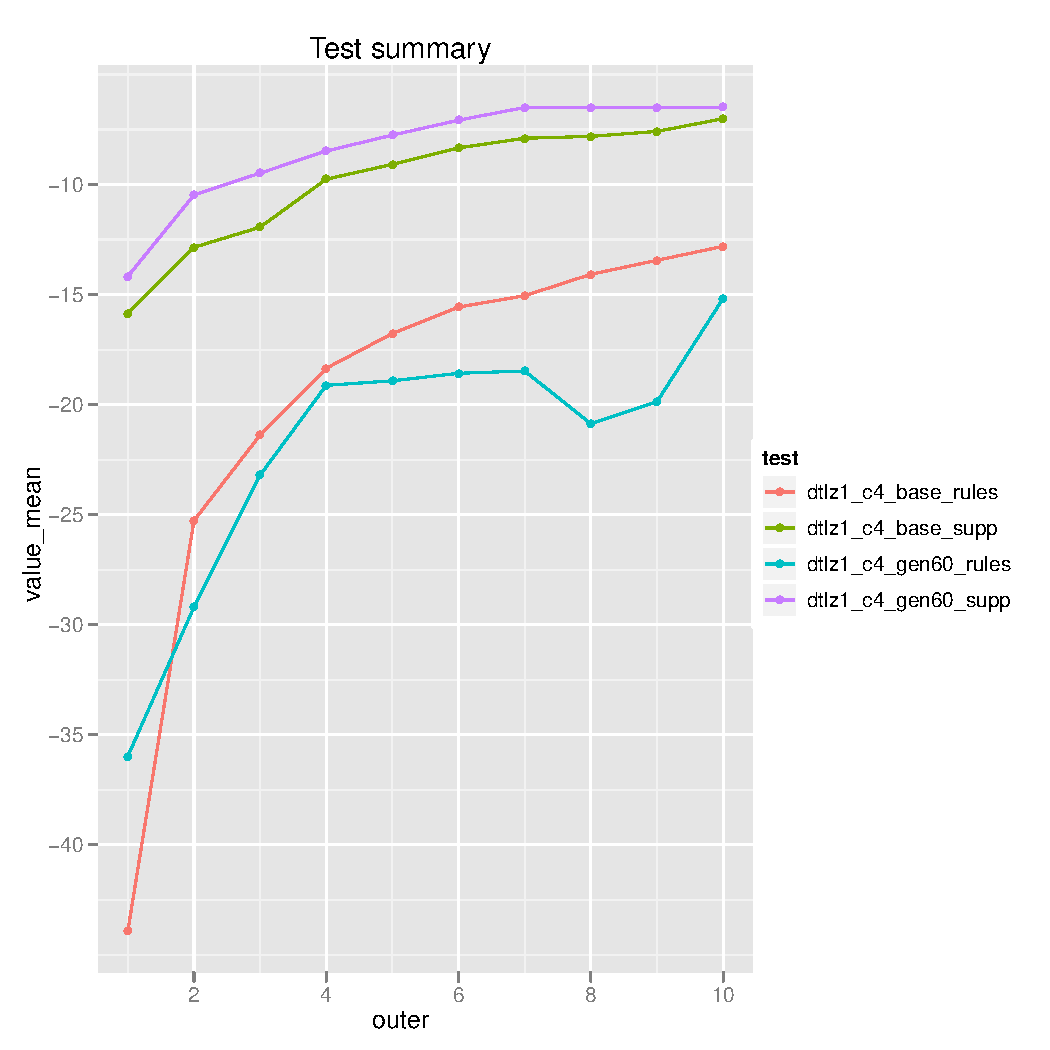
\includegraphics[scale=0.53]{exp/uncert/dtlz1_c4_perf1}
      \label{dtlz1_c4_perf1}
    }
    \subfloat{
      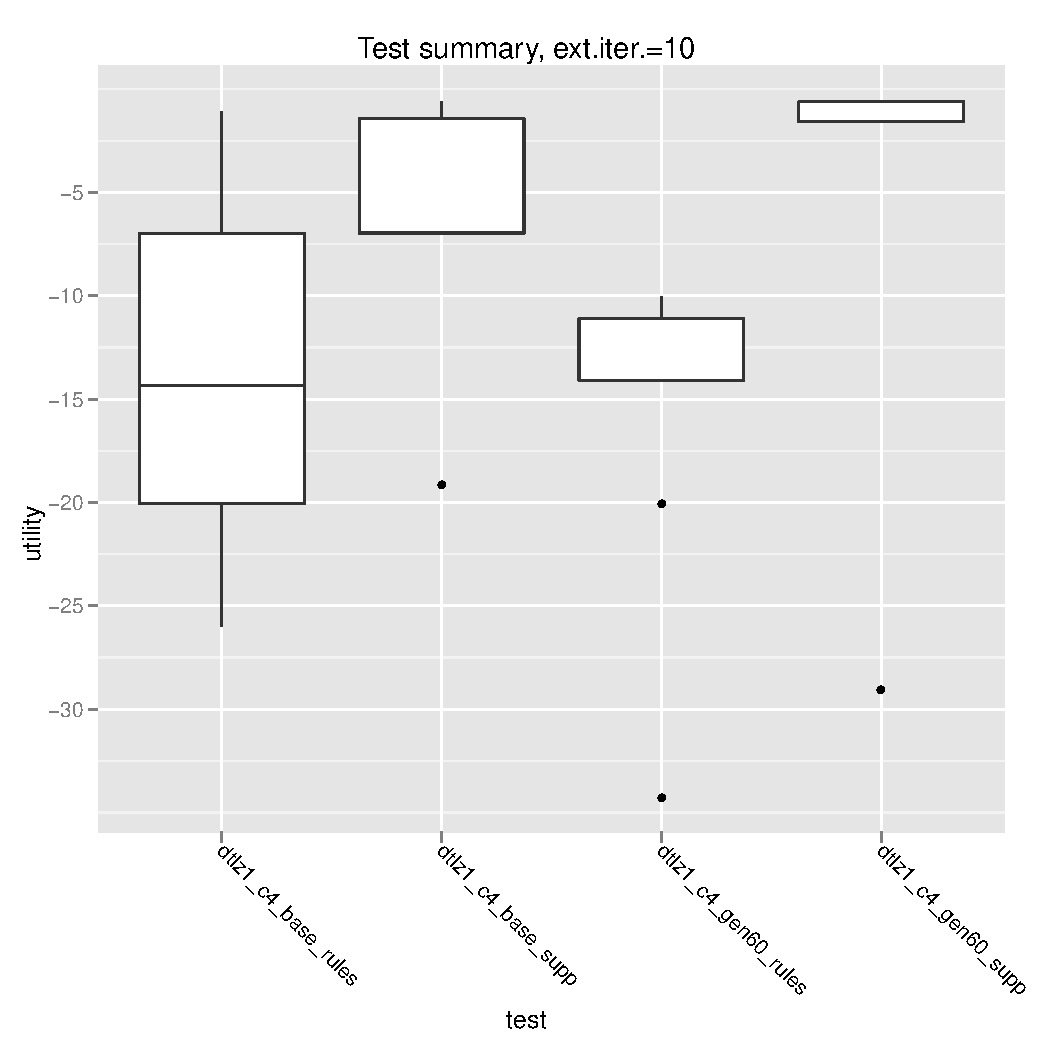
\includegraphics[scale=0.53]{exp/uncert/dtlz1_c4_perf1b}
      \label{dtlz1_c4_perf1b}
    }
  }
  \caption{Performance comparison on the four-criteria DTLZ1 problem}
  \label{dtlz1_c4_perf}
\end{figure}

\begin{figure}
  \centering
  \makebox[\textwidth]{
    \subfloat{
      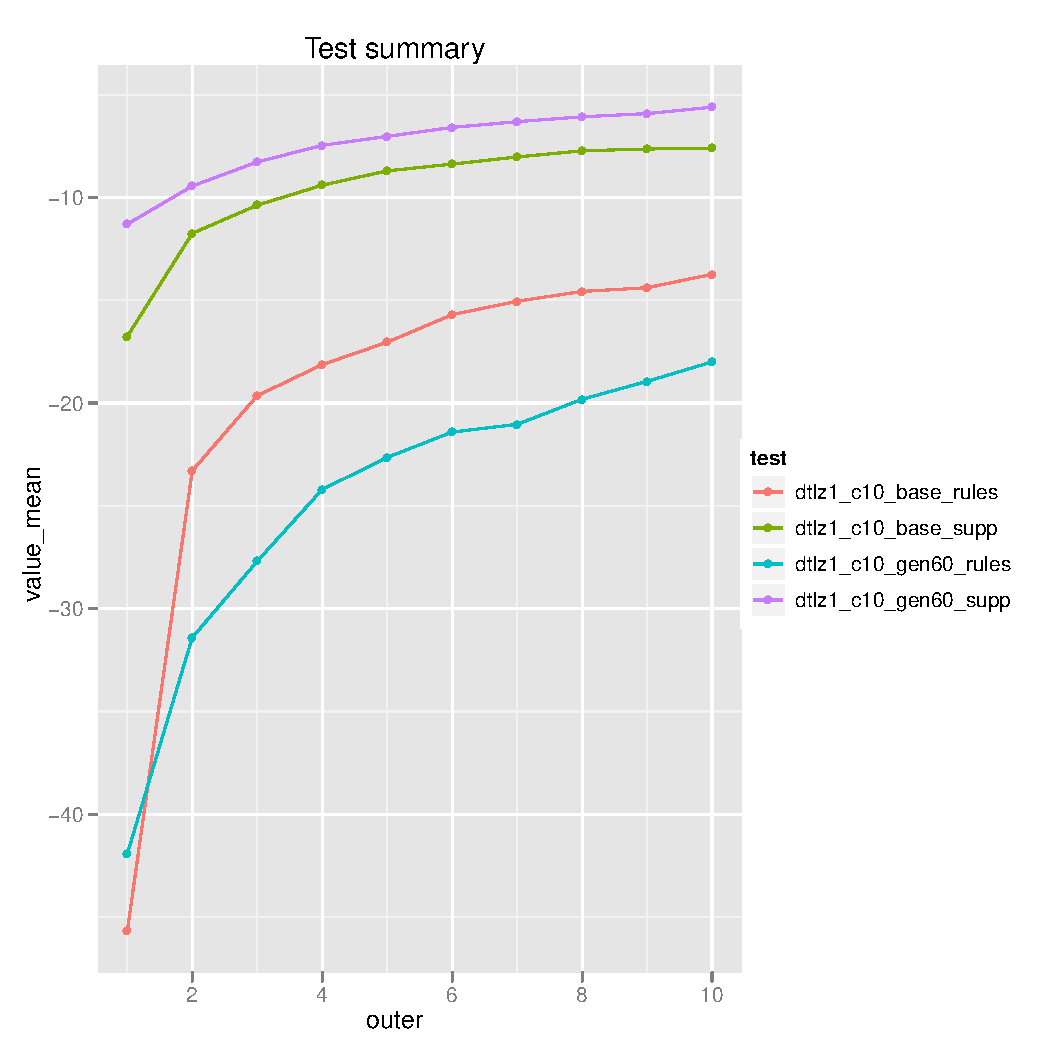
\includegraphics[scale=0.53]{exp/uncert/dtlz1_c10_perf1}
      \label{dtlz1_c10_perf1}
    }
    \subfloat{
      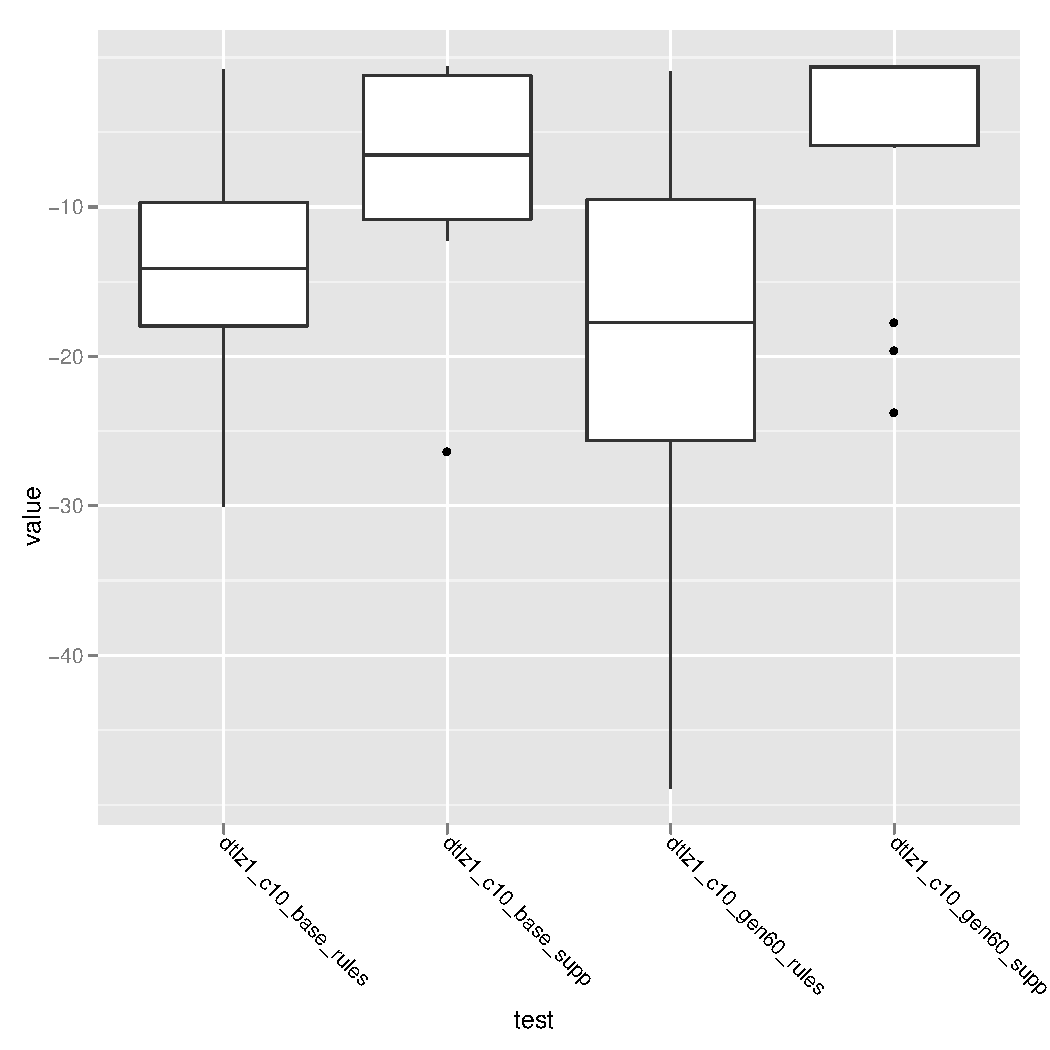
\includegraphics[scale=0.53]{exp/uncert/dtlz1_c10_perf1b}
      \label{dtlz1_c10_perf1b}
    }
  }
  \caption{Performance comparison on the ten-criteria DTLZ1 problem}
  \label{dtlz1_c10_perf}
\end{figure}

\begin{figure}
  \centering
  \makebox[\textwidth]{
    \subfloat{
      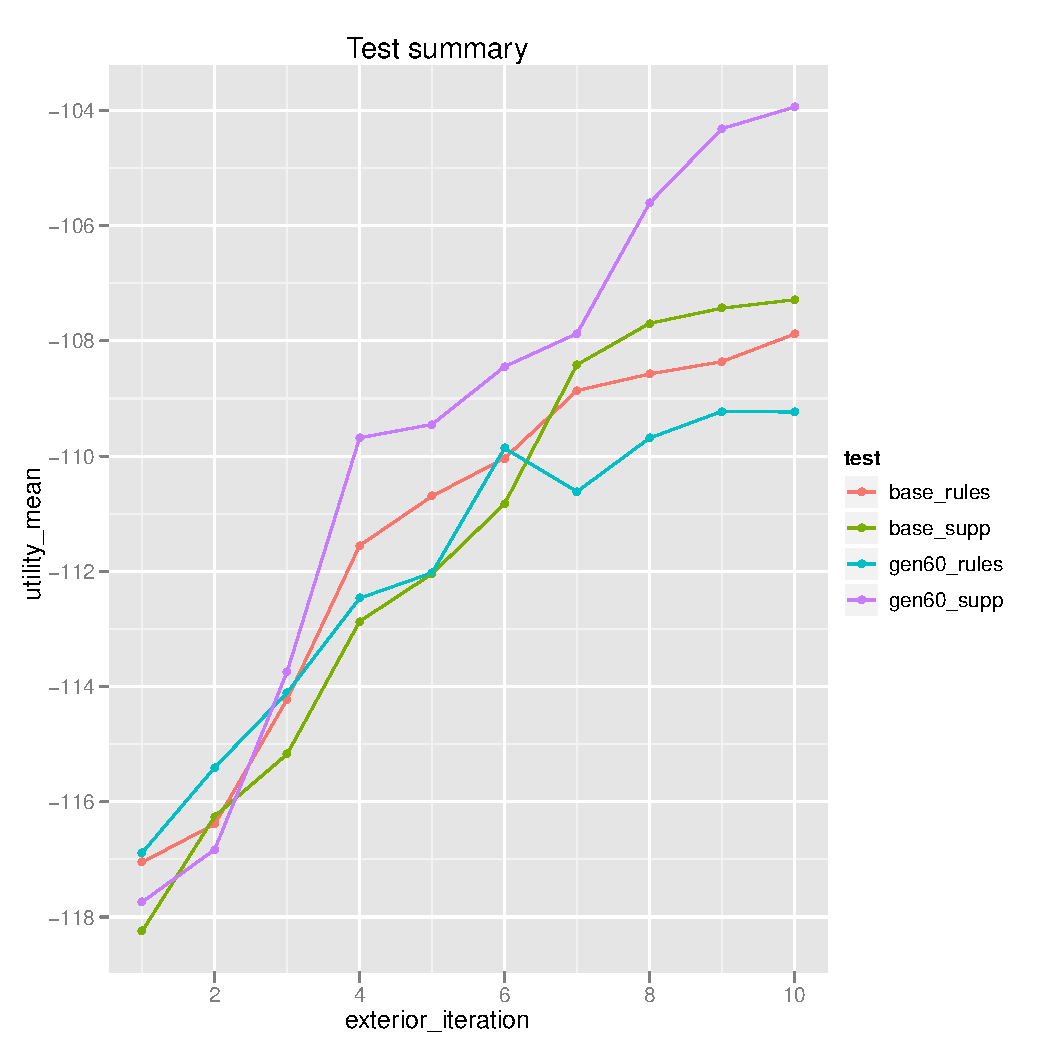
\includegraphics[scale=0.53]{exp/uncert/dtlz7_c4_perf1}
      \label{dtlz7_c4_perf1}
    }
    \subfloat{
      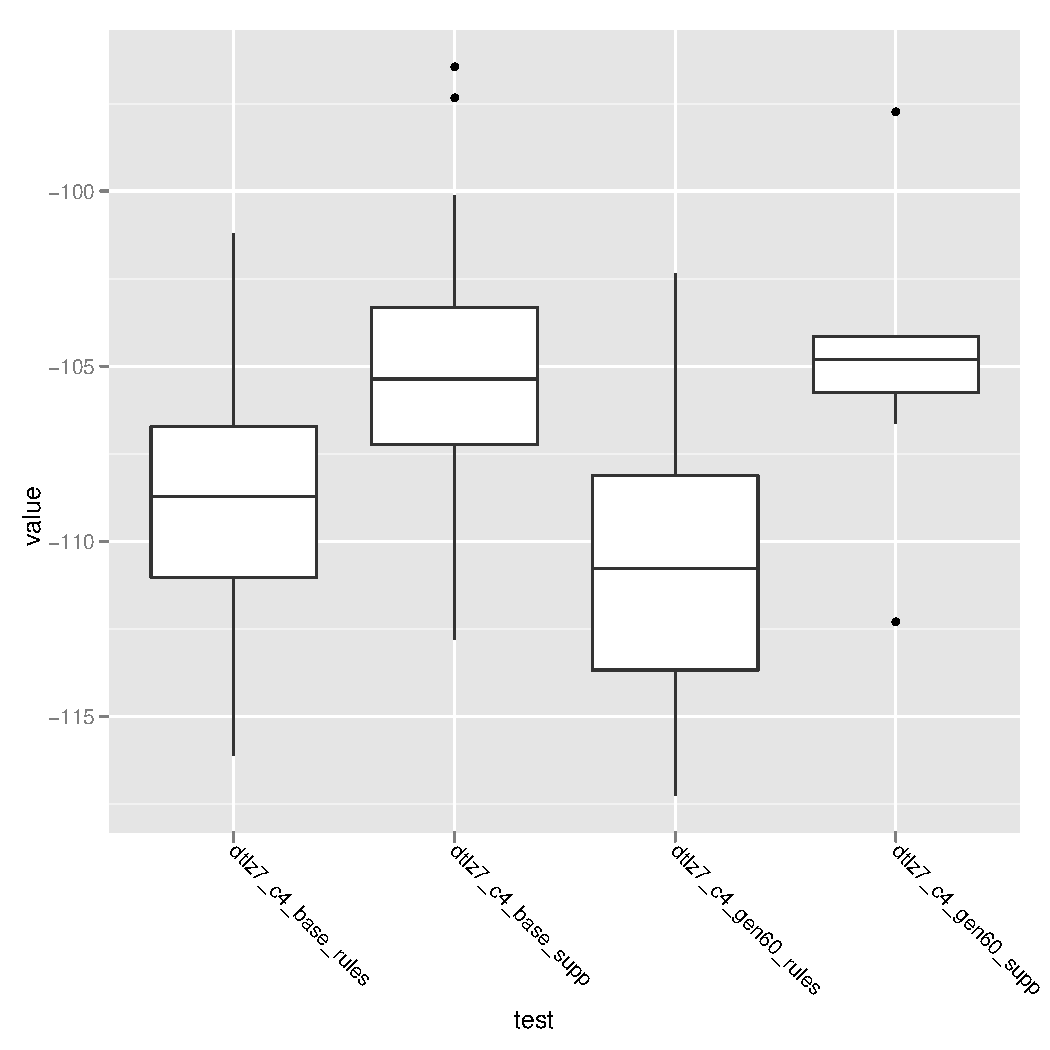
\includegraphics[scale=0.53]{exp/uncert/dtlz7_c4_perf1b}
      \label{dtlz7_c4_perf1b}
    }
  }
  \caption{Performance comparison on the four-criteria DTLZ7 problem}
  \label{dtlz7_c4_perf}
\end{figure}

TODO: Data table and conclusions
\clearpage{}

\subsection{The importance of parameters}
\clearpage{}

\subsection{Noise in the DM's decisions}

In order to check impact of a noise in DM's decisions experiments were
performed. The results are presented in figure~\ref{noise}.

The effect of the noise starts to be an important factor only in case of
medium (noise$_5$) and major (noise$_6$). So the situation is similar to the
impact on problems defined without uncertainty. Even if one adds the interval
coefficients to the problem the solution is still robust with respect to the
noise.


\begin{figure}
  \centering
  \makebox[\textwidth]{
    \subfloat[Mix problem]{
      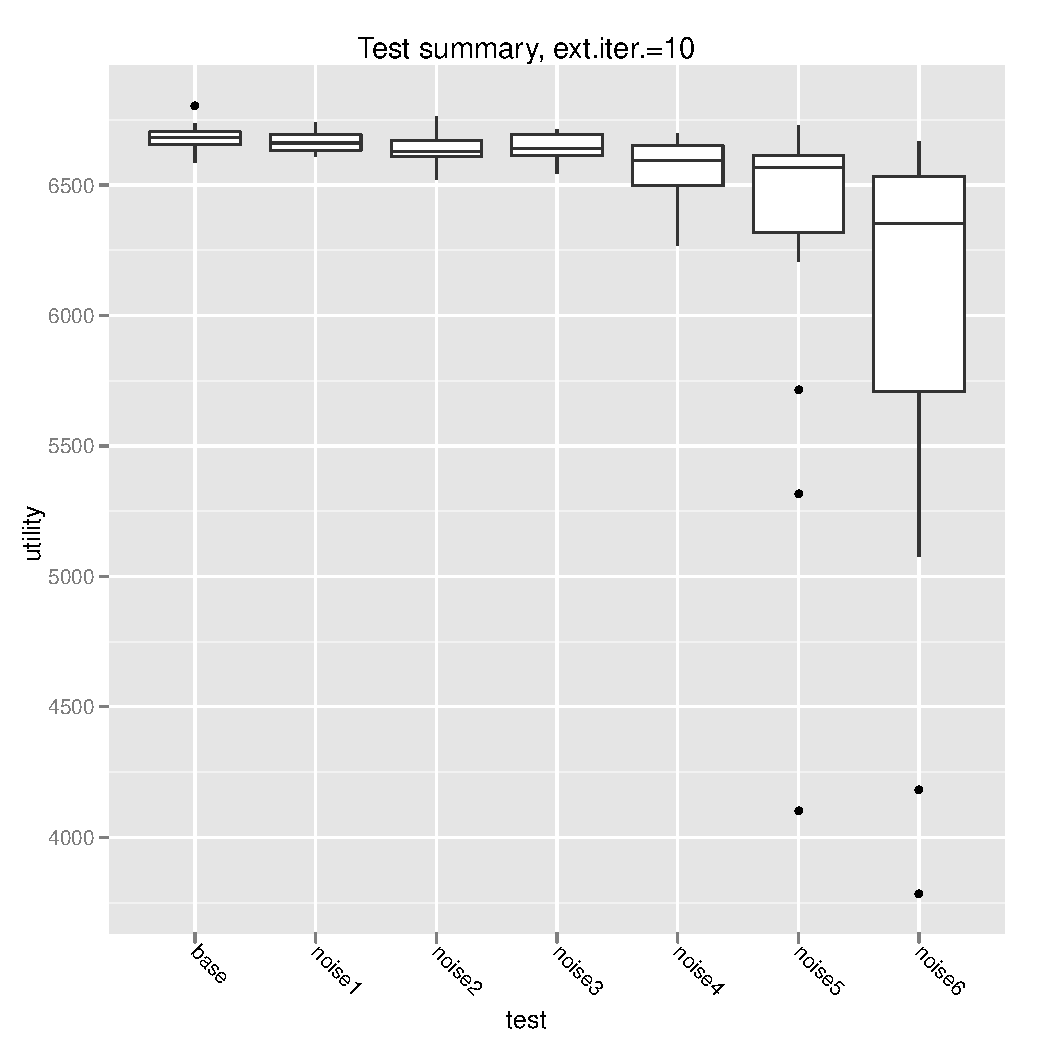
\includegraphics[scale=0.53]{exp/uncert/pres_noise}
      \label{pres_noise}
    }
    \subfloat[DTLZ1 four-criteria]{
      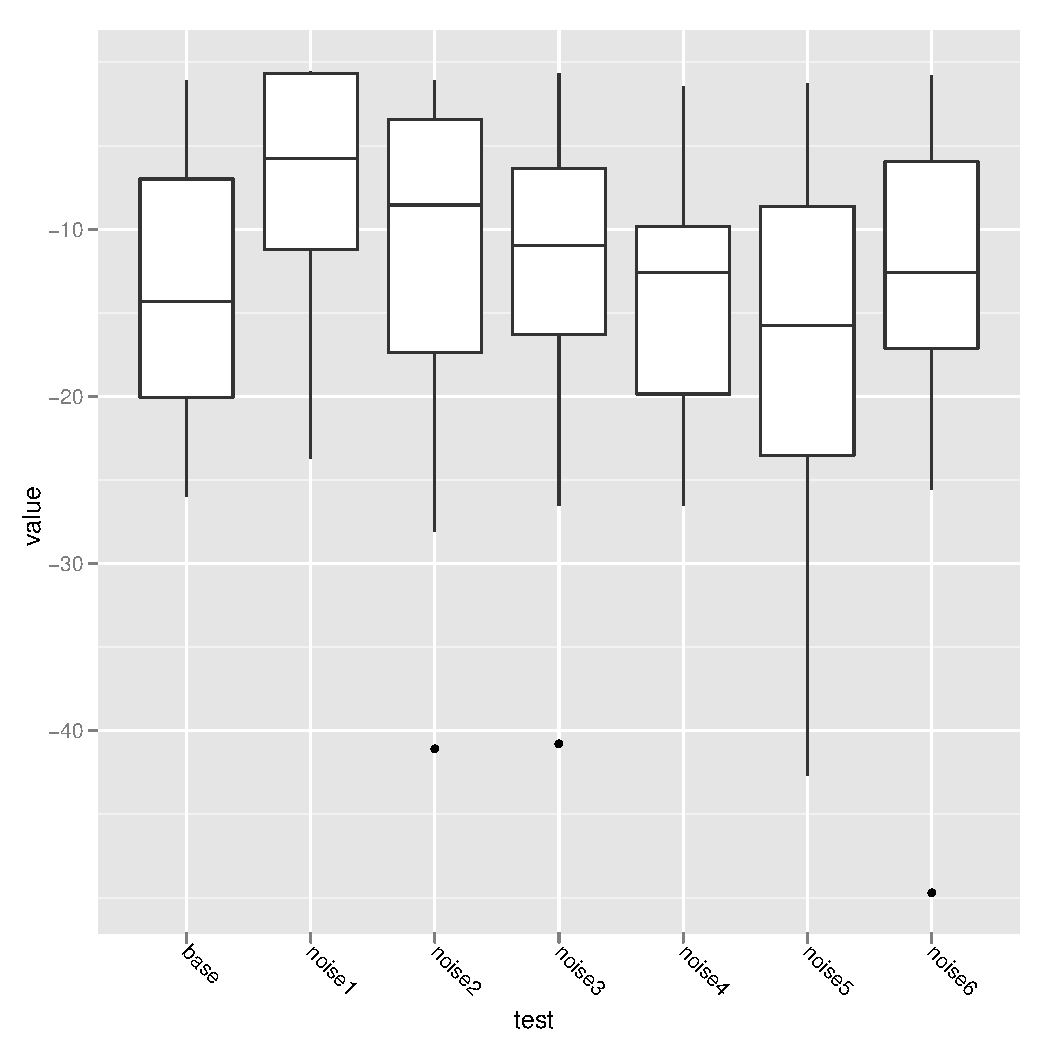
\includegraphics[scale=0.53]{exp/uncert/dtlz1_c4_noise}
      \label{dtlz1_c4_noise}
    }
  }
  \makebox[\textwidth]{
    \subfloat[DTLZ1 ten-criteria]{
      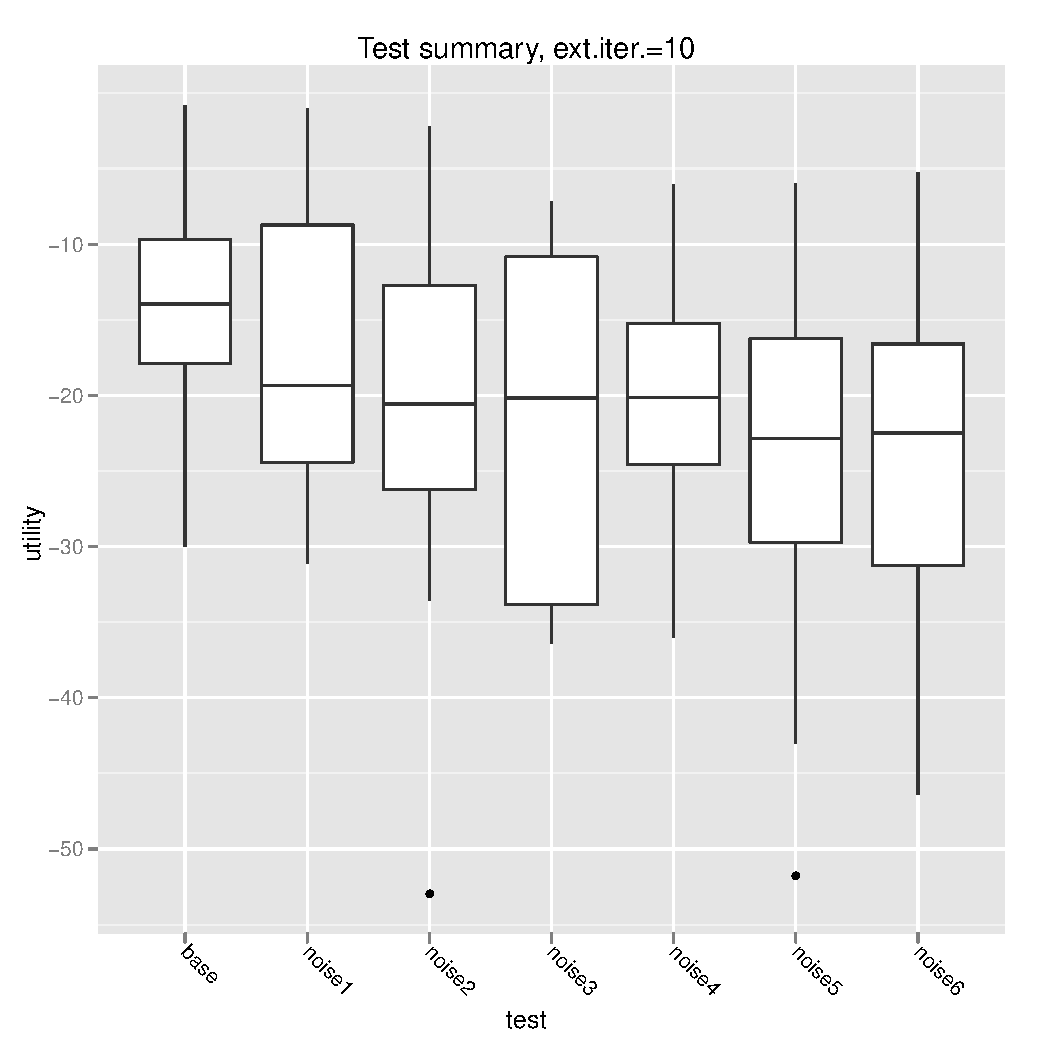
\includegraphics[scale=0.53]{exp/uncert/dtlz1_c10_noise}
      \label{dtlz1_c10_noise}
    }
    \subfloat[DTLZ7 four-criteria]{
      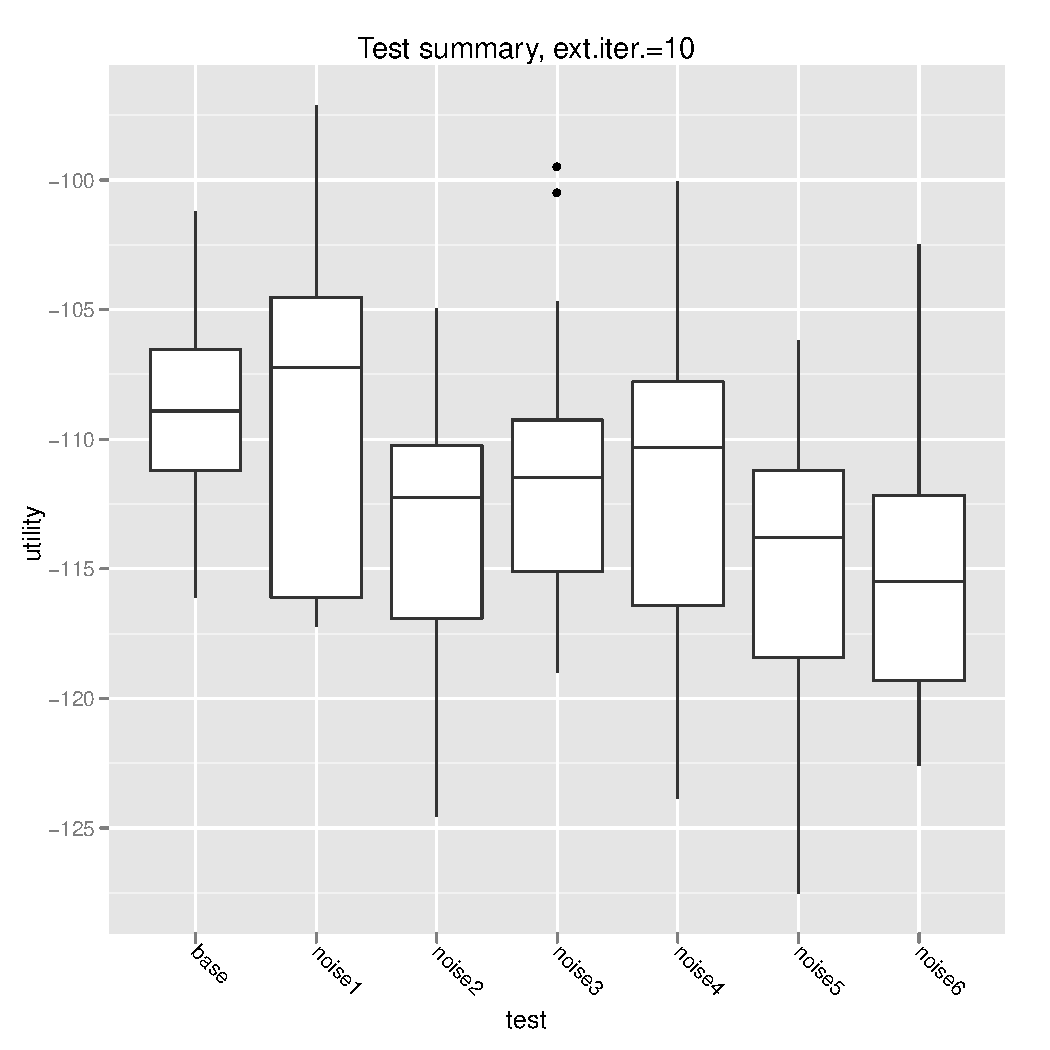
\includegraphics[scale=0.53]{exp/uncert/dtlz7_c4_noise}
      \label{dtlz7_c4_noise}
    }
  }
  \caption{Effect of noise in DM's decisions}
  \label{noise}
\end{figure}


\clearpage{}
